\documentclass[11pt,a4paper]{article}
\usepackage[margin=2cm]{geometry}
\usepackage[T1]{fontenc}
\usepackage{amsmath,amssymb}
\usepackage{graphicx}
\usepackage{booktabs}
\usepackage{array}
\usepackage{url}
\usepackage{enumitem}
\setlist{itemsep=1pt,topsep=3pt}
\newcommand{\Rref}{R_{\mathrm{ref}}}
\newcommand{\Zx}{Z_x}
\newcommand{\Vmid}{V_{\mathrm{mid}}}

\title{Digital Impedance Meter using a Raspberry Pi Pico 2}
\author{Prabhuparth Choudhar \\ Roll No.\ 24EE01065}
\date{13 November 2026}

\begin{document}
\maketitle
\noindent Measurements and Electrical Instruments (MEI) course project, IIT Bhubaneswar

\section{Objective}
Build an instrument that measures an unknown impedance $\Zx$ (R, L or C) at 125, 250, 500 and 1000~Hz, using a Raspberry Pi Pico 2, a reference resistor, op-amp buffers and software (lock-in detection and calibration). Check the design in simulation first, then build it on a breadboard and test it.

Scope of this report: one circuit (a resistive divider with a reference resistor), simulated in LTspice, built on a breadboard, and tested with resistors and capacitors.

\section{Measurement principle}
A reference resistor $\Rref$ is in series with the unknown $\Zx$. The Pico drives $V_1$ (sine, PWM through a filter and buffer). The other end of $\Zx$ is held at $V_2 = 1.65$~V DC. The ADC reads $V_1$ and the middle node $\Vmid$.

Current: $I = (V_1 - \Vmid)/\Rref$. With $H = \Vmid / V_1$ (complex ratio of the AC parts; $V_2$ is DC, so it drops out):
\begin{equation}
  \Zx = \Rref \, \frac{H}{1-H}
\end{equation}
$R = \mathrm{Re}(\Zx)$, $X = \mathrm{Im}(\Zx)$, $L = X/\omega$, $C = -1/(\omega X)$, $\omega = 2\pi f$. The result is a ratio, so the exact signal amplitude and ADC reference do not matter, only $\Rref$ and the ADC channel match do. Accuracy is best when $|\Zx|$ is close to $\Rref$, so $\Rref$ is selectable (100~$\Omega$, 1~k$\Omega$, 9.9~k$\Omega$, 100.4~k$\Omega$ measured values; one fitted at a time).

\section{Hardware circuit}
\begin{figure}[h]
  \centering
  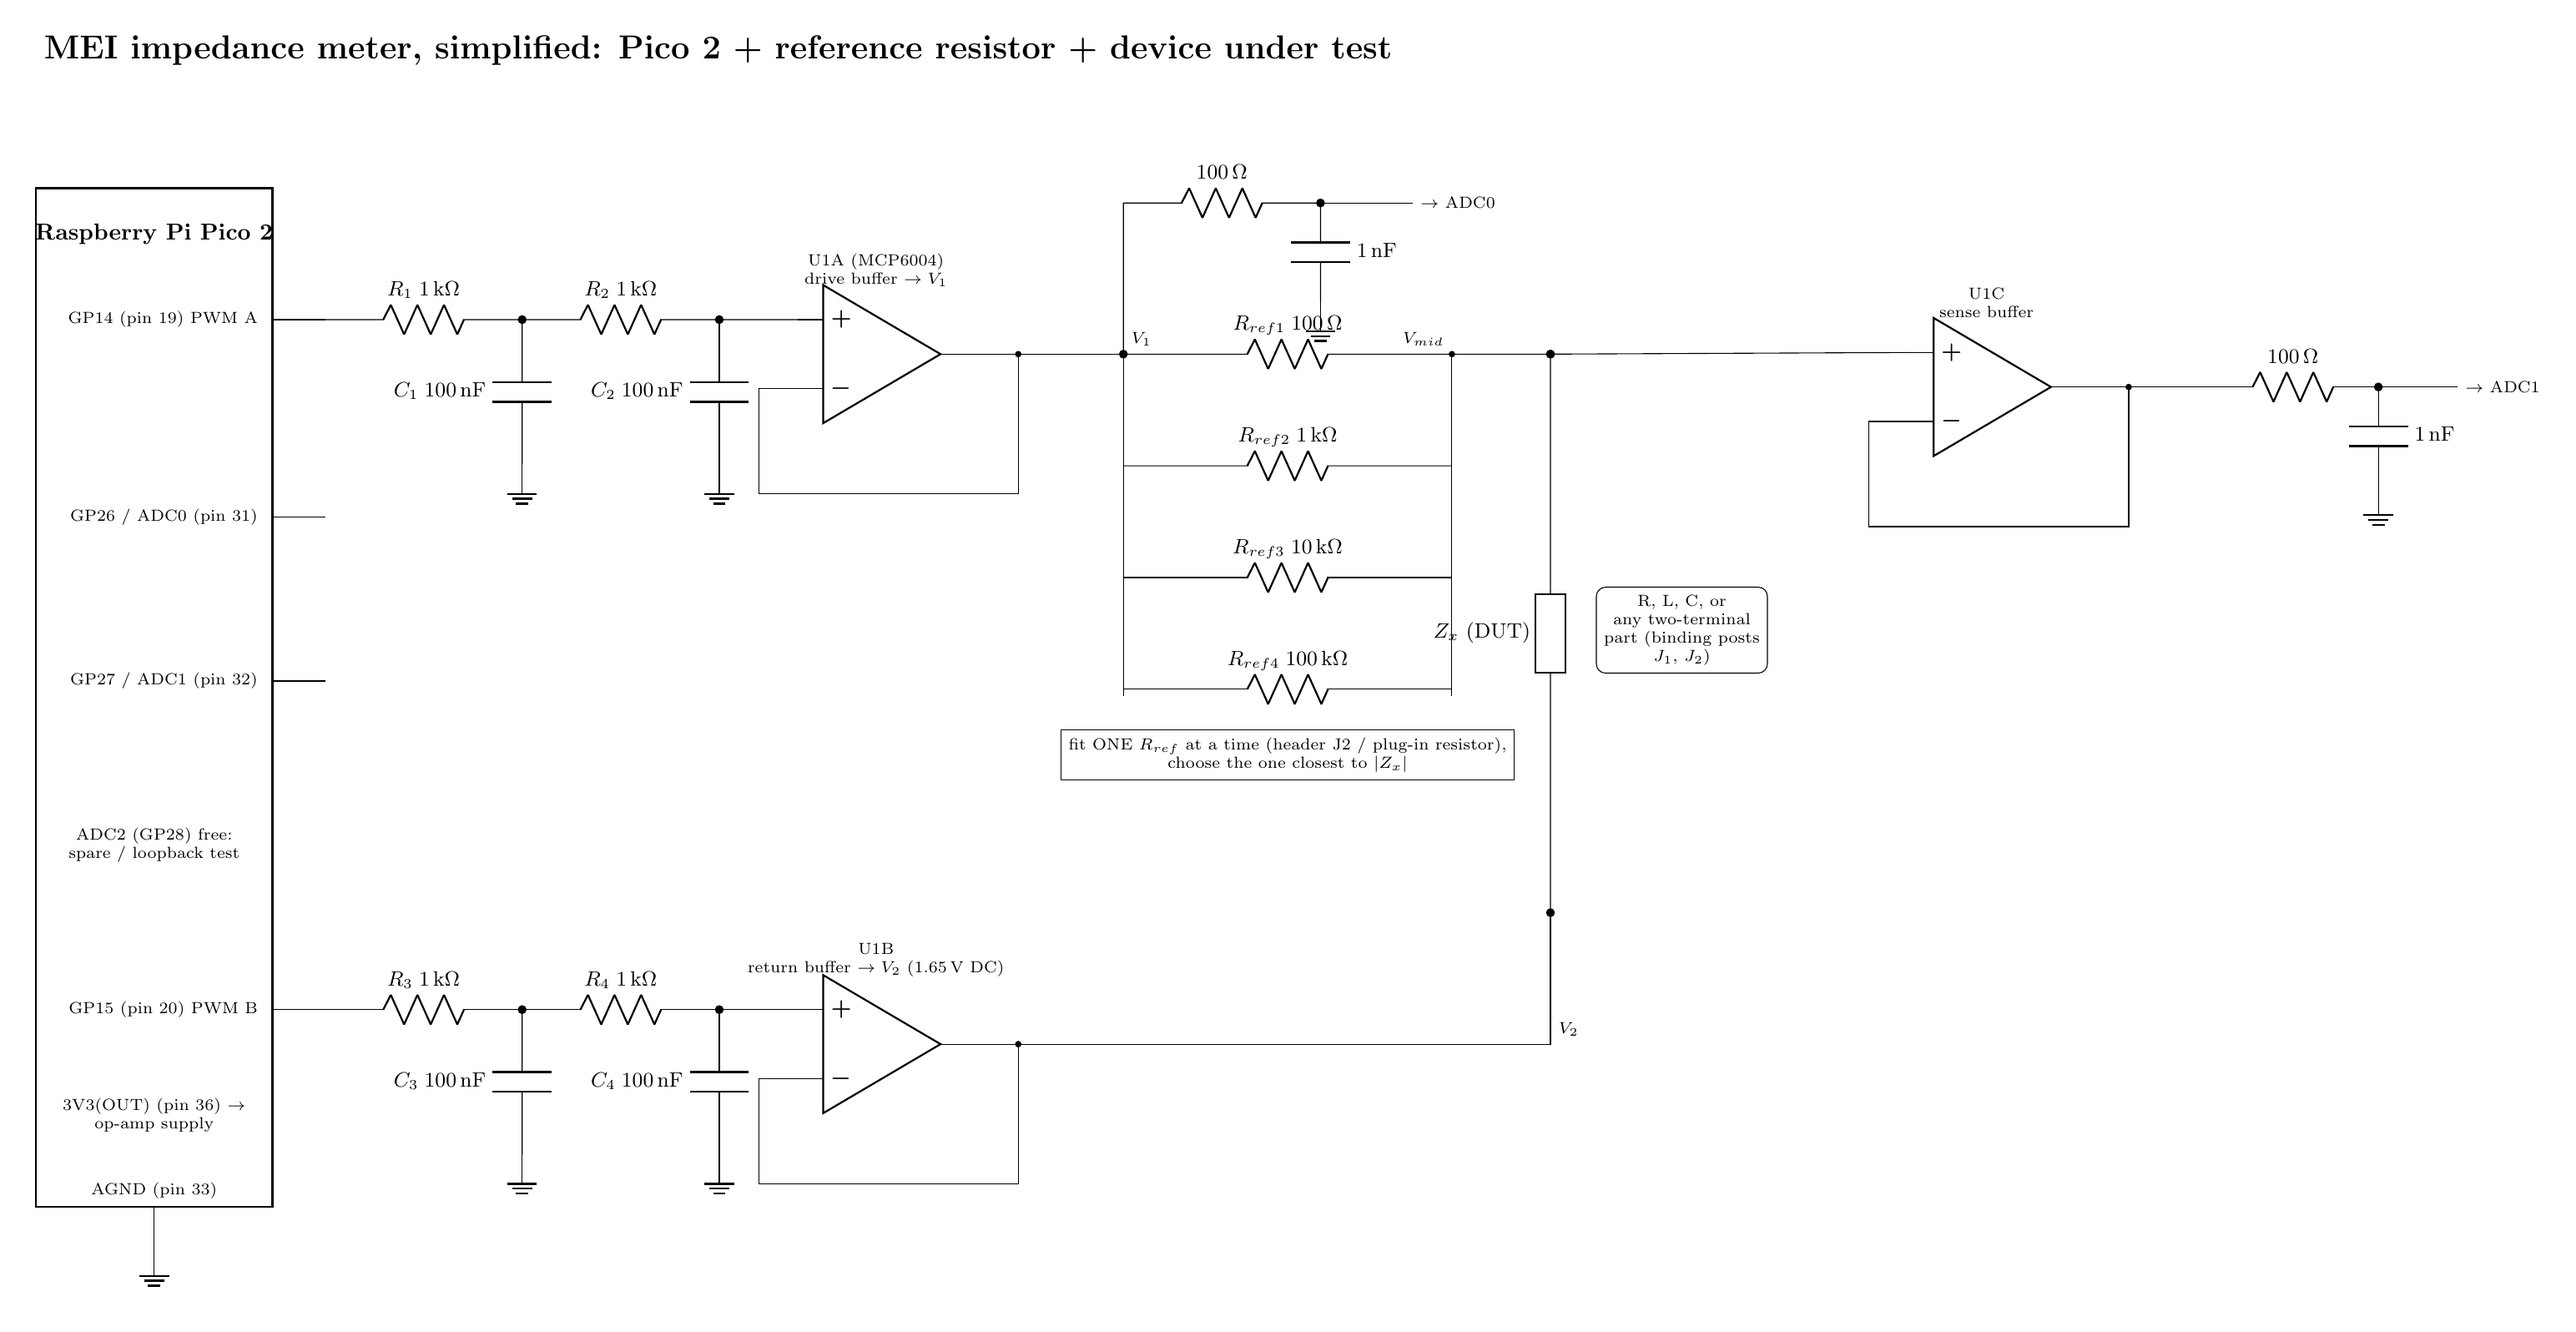
\includegraphics[width=\textwidth]{fig/hw_circuit.png}
  \caption{Circuit as built. Full-size drawing: \texttt{hardware/mei\_circuit\_divider.pdf}.}
\end{figure}
\begin{itemize}
  \item \textbf{Drive:} GP14 (PWM A) $\to$ two-stage RC filter (1~k$\Omega$ + 100~nF, twice) $\to$ U1A follower $\to V_1$.
  \item \textbf{Return:} GP15 (PWM B) $\to$ same filter $\to$ U1B follower $\to V_2$ (about 1.65~V DC).
  \item \textbf{Divider:} $V_1$ -- $\Rref$ -- $\Vmid$ -- $\Zx$ -- $V_2$.
  \item \textbf{Sensing:} ADC0 (GP26) reads $V_1$ through 100~$\Omega$ + 1~nF. ADC1 (GP27) reads $\Vmid$ through the U1C buffer and 100~$\Omega$ + 1~nF. ADC2 was used only for loopback tests.
  \item \textbf{Op-amp:} MCP6004 (quad, rail-to-rail), supplied from the Pico 3V3. AGND is the star ground. GPIO23 is driven high to put the Pico supply in PWM mode (lower ADC noise).
  \item \textbf{Measured parts (multimeter):} R1 = R2 = 1.00~k$\Omega$, R3 = R4 = 0.99~k$\Omega$, $\Rref$ = 100, 1000, 9900, 100400~$\Omega$. The 1~nF ADC capacitors were not measured.
\end{itemize}

\subsection*{Firmware and software}
\begin{itemize}
  \item MicroPython on the Pico. The sine is made by changing PWM duty in 5 to 40 steps per cycle. At 500~Hz it is 10 steps of 200~$\mu$s.
  \item ADC0 and ADC1 are read one after the other, not at the same instant. Each sample has a microsecond timestamp, and the phasors are computed with the real times (this removes the skew, about 19~$\mu$s or $3.5^\circ$ at 500~Hz).
  \item Lock-in: the host computes complex $V_1$ and $\Vmid$ by correlation with sine and cosine at the drive frequency, then $H$ and $\Zx$.
  \item Calibration (per $\Rref$ and frequency): $H_{\mathrm{meas}} = k\,H_{\mathrm{true}} + c$, with complex $k$ and $c$ fitted from a short, an open circuit and a known resistor.
  \item Model identification: the tool fits R, L, C, R+L, R+C, R$\|$C and R$\|$L at all four frequencies and reports the simplest model whose fit error is under 2~\%.
  \item Code: \texttt{firmware/imeter.py} (main tool), \texttt{lockin.py}, \texttt{analyze.py}, \texttt{dc\_check.py}, \texttt{config.py}, \texttt{cal.json}.
\end{itemize}

\section{Simulation}
\subsection{LTspice model}
\begin{figure}[h]
  \centering
  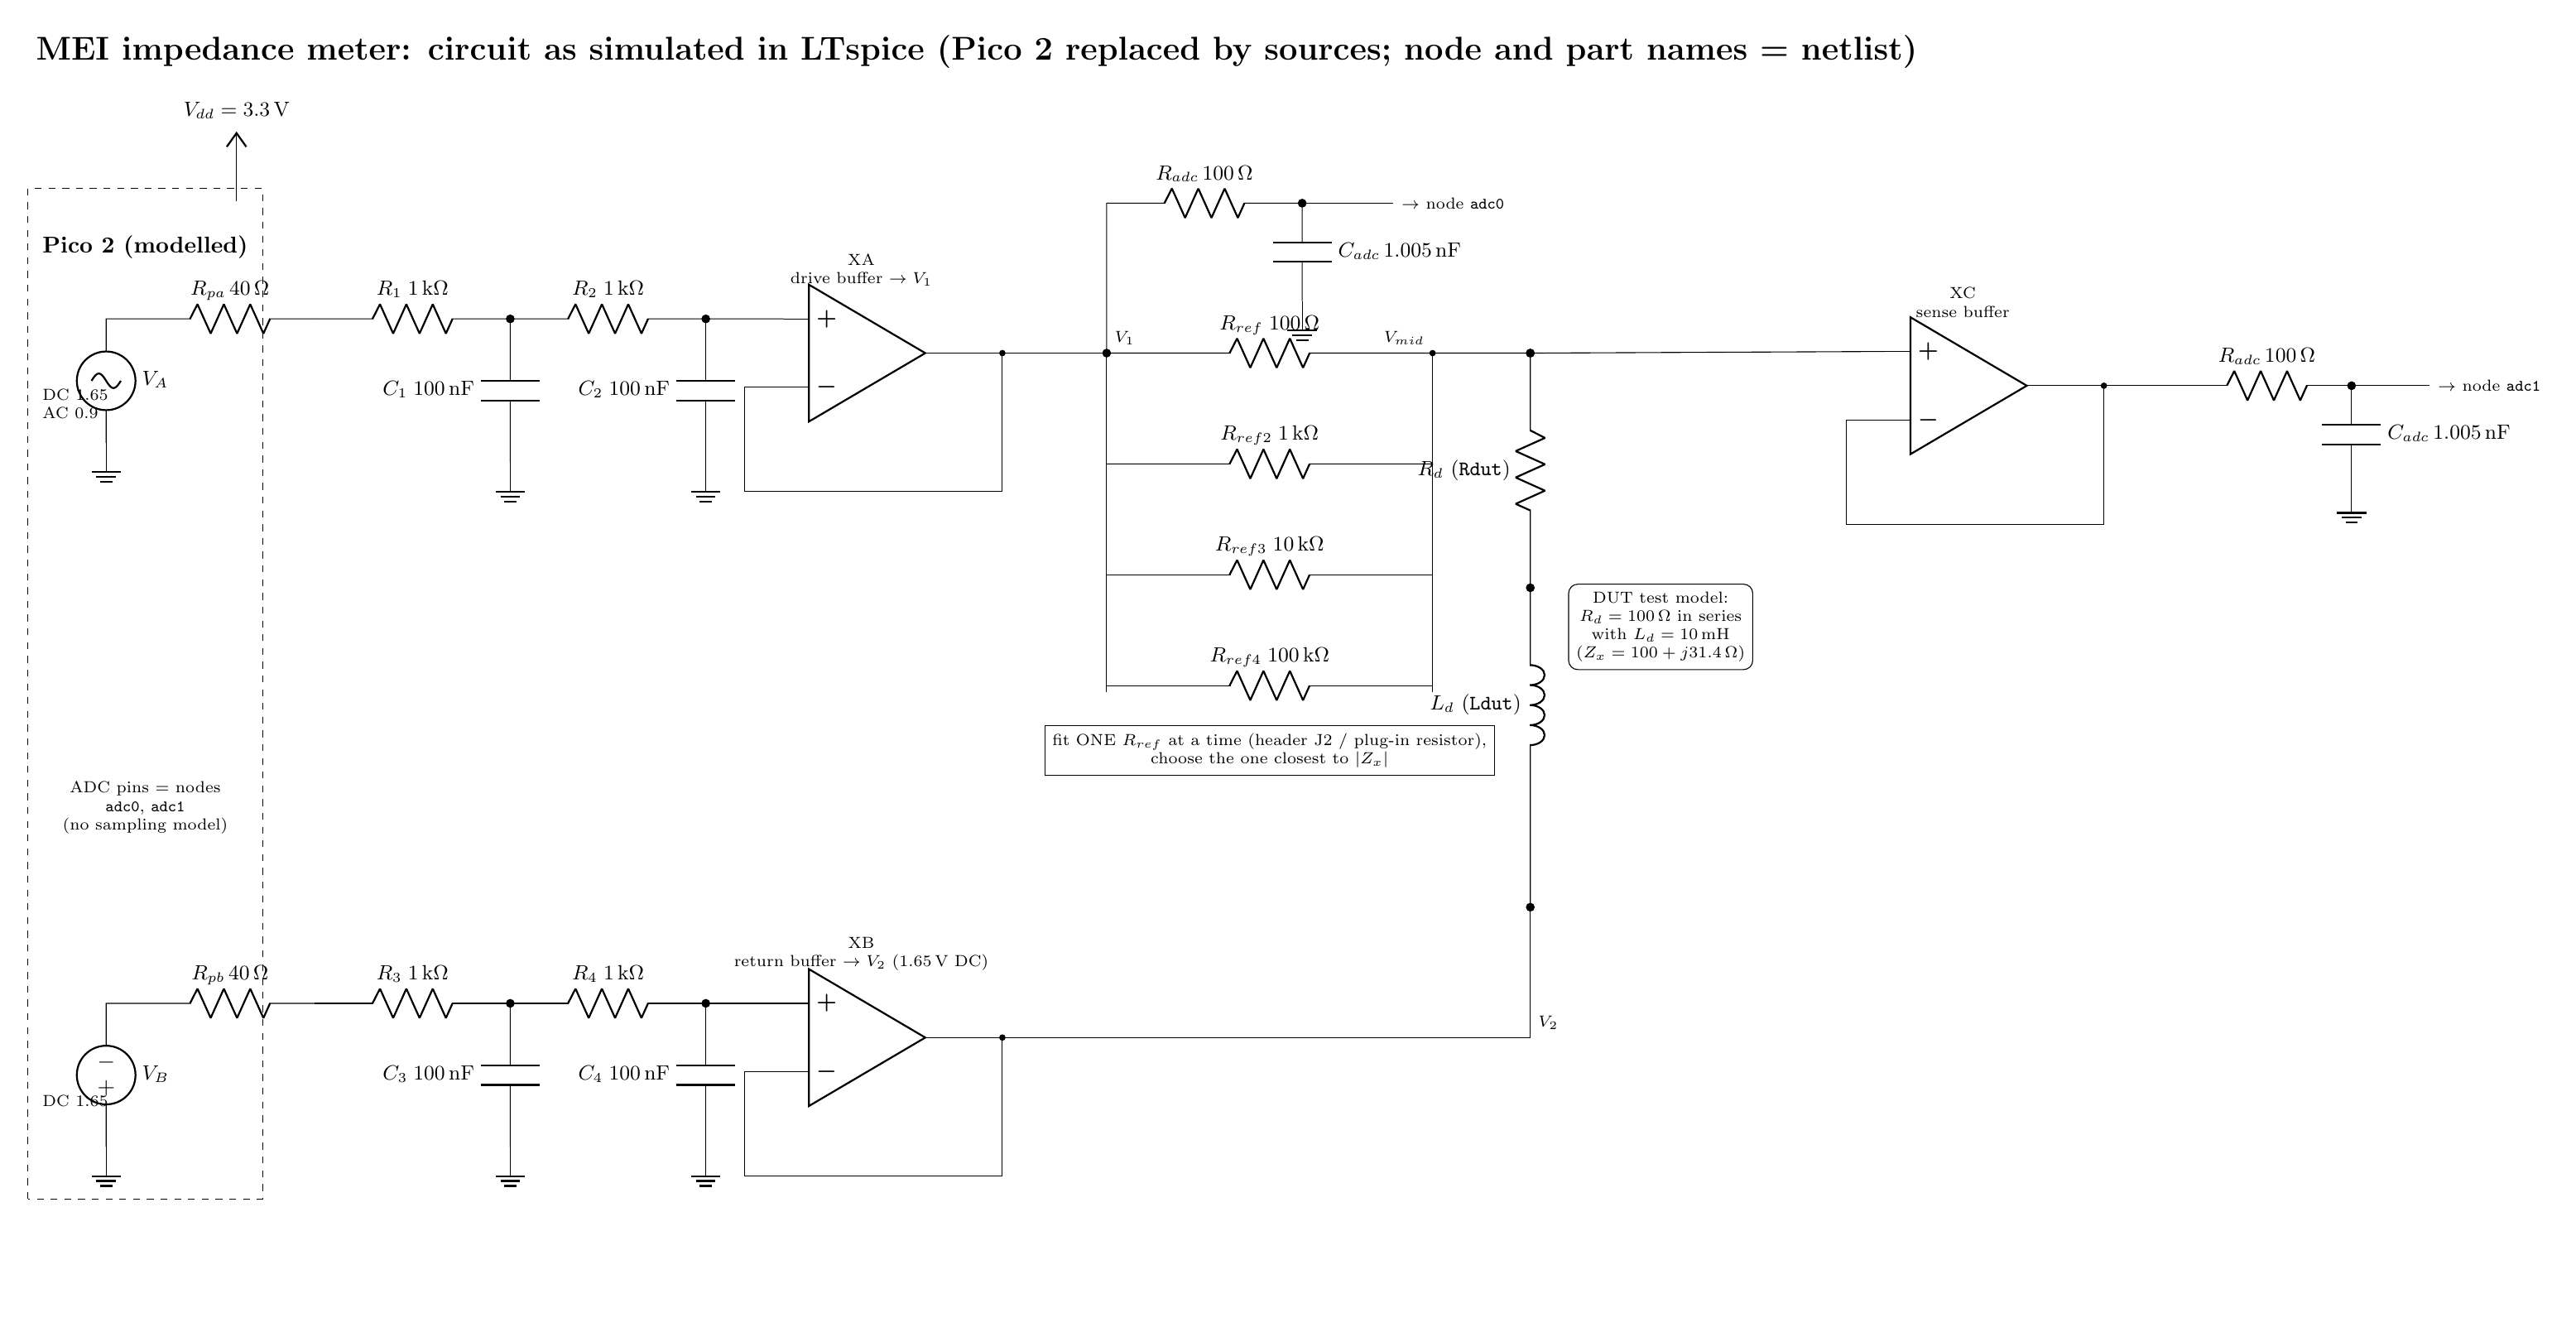
\includegraphics[width=\textwidth]{fig/sim_circuit.png}
  \caption{Circuit as simulated in LTspice (file \texttt{simulation/ltspice/Impedence\_Measurement.asc}). Full-size drawing: \texttt{simulation/ltspice/mei\_circuit\_ltspice.pdf}.}
\end{figure}
\begin{itemize}
  \item The Pico pins are replaced by sources: $V_A$ = 1.65~V DC + 0.9~V AC at 500~Hz, $V_B$ = 1.65~V DC, each with 40~$\Omega$ pin resistance. ADC pins are plain nodes (\texttt{adc0}, \texttt{adc1}), with no sampling model.
  \item Same filters, buffers, $\Rref$ and ADC input networks as the hardware. $V_{dd}$ = 3.3~V.
  \item Op-amp: simple macro-model (\texttt{.subckt opamp2}): $A_{vol}$ = 100~k, GBW = 1~MHz, slew 0.6~V/$\mu$s, output swing within 25~mV of the rails, $R_{out}$ = 100~$\Omega$.
  \item DUT: $R_d$ in series with $L_d$ (a resistor uses $L_d$ = 1~nH). Seven cases are stepped with \texttt{.step param case 1 7 1}; $\Rref$, $R_d$ and $L_d$ come from a table in the schematic. Cases 2 to 6 are the resistors used in hardware runs 1, 4, 6, 9, 11.
  \item Analysis: \texttt{.ac list 125 250 500 1000}. $\Zx$ is computed as $\Rref \cdot V(\texttt{adc1}) / (V(\texttt{adc0}) - V(\texttt{adc1}))$ with \texttt{simulation/ltspice/extract\_z.py}, which reads the \texttt{.raw} file and writes \texttt{results.csv}.
\end{itemize}

\subsection{LTspice results}
Results at 500~Hz. The full table (all seven cases at 125, 250, 500 and 1000~Hz, true and computed R and X) is in \texttt{simulation/ltspice/results.csv}.
\begin{center}
\small
\begin{tabular}{rllrrr}
\toprule
Case & DUT (true) & $\Rref$ & $|V(\texttt{adc1})|$ & $\Zx$ computed ($\Omega$) & R error \\
\midrule
1 & 100~$\Omega$ + 10~mH & 100~$\Omega$ & 353 mV & 100.05 + j31.37 & +0.0473~\% \\
2 & 6.15~k$\Omega$ & 9.9~k$\Omega$ & 261 mV & 6149.90 $-$ j4.94 & $-0.0016$~\% \\
3 & 4.7~k$\Omega$ & 9.9~k$\Omega$ & 220 mV & 4699.93 $-$ j3.42 & $-0.0015$~\% \\
4 & 2.664~k$\Omega$ & 9.9~k$\Omega$ & 145 mV & 2663.97 $-$ j1.64 & $-0.0012$~\% \\
5 & 220~$\Omega$ & 1~k$\Omega$ & 123 mV & 220.00 $-$ j0.08 & $-0.0003$~\% \\
6 & 2~k$\Omega$ & 1~k$\Omega$ & 455 mV & 1999.94 $-$ j2.95 & $-0.0031$~\% \\
7 & 1~k$\Omega$ + 100~mH & 9.9~k$\Omega$ & 66 mV & 1000.18 + j313.66 & +0.0180~\% \\
\bottomrule
\end{tabular}
\end{center}
R error is small in every case (largest $+0.19$~\% for case 1 at 1~kHz). Over all 28 points the error of $\Zx$ is under 0.3~\% of $|\Zx|$; the largest is case 6 at 1~kHz ($X = -5.9~\Omega$ on 2~k$\Omega$). Remaining error comes from the finite op-amp bandwidth (GBW 1~MHz) and the 100~$\Omega$ + 1~nF ADC input filters.

\textbf{Reactance of the resistor cases.} In cases 2 to 6 the true reactance is about zero (1~nH), but the computed $X$ is negative and grows with frequency and with $R$ (for 6.15~k$\Omega$: $-1.2~\Omega$ at 125~Hz, $-9.9~\Omega$ at 1~kHz). This is a phase error of about $-2\times10^{-4}$~rad at 125~Hz, a delay of about 0.25~$\mu$s between the adc0 and adc1 paths. It is probably the lag of the extra sense buffer (U3, GBW 1~MHz, about 0.16~$\mu$s) in the adc1 path; I did not test this separately. The 19~$\mu$s sampling skew of the real ADC is much larger and is corrected in firmware with timestamps.

Signal level: $V(\texttt{adc0})$ is 0.68~V peak, not the 0.9~V set at the source, because the two-stage RC filter attenuates 500~Hz (gain about 0.77). $V(\texttt{adc1})$ is smallest when $\Rref$ is much larger than $|\Zx|$ (case 7: 66~mV peak with $\Rref$ 9.9~k$\Omega$, $|\Zx|$ about 1.05~k$\Omega$). The simulation has no ADC noise (hardware: about 0.5~mV rms per sample), so $\Rref$ should be chosen close to $|\Zx|$.

\subsection{Other simulations done}
\begin{itemize}
  \item \textbf{Stage 0} (Python phasor Monte Carlo, \texttt{simulation/stage0/}): showed that resistor tolerance sets the accuracy, that the divider reading is better than the bridge-difference reading, that skew between ADC channels must be compensated, and that ADC channel gain mismatch should be below about 0.02~\% after loopback.
  \item \textbf{Co-simulation} (\texttt{simulation/cosim/}): a Python model of the Pico running inside an ngspice transient simulation (libngspice), with 12-bit ADC at 480~kS/s, noise, and real 150~kHz PWM. It was run for a \textbf{Wheatstone} module, not for the built divider. Results with 0.1~\% resistors: reading error 0.10~\% (std) for the bridge reading and 0.06~\% for the divider reading. With 1~\% resistors: 1.05~\% and 0.62~\%. Pin resistance and ADC noise had no visible effect, because the measurement is a ratio. Not modelled: ADC INL/DNL, sampling kick-back, strays, temperature. Datasheet values used: RP2350 ADC and GPIO tables, Microchip MCP6004 macro-model.
\end{itemize}

\section{Hardware results}
\subsection{ADC and front-end checks (11 Nov 2026)}
\begin{center}
\small
\begin{tabular}{p{5.2cm}p{10.5cm}}
\toprule
Check & Result \\
\midrule
ADC offset, input shorted to AGND (2000 samples) & ADC0 4.54~mV, ADC1 4.66~mV, ADC2 4.60~mV; noise 0.51 to 0.58~mV rms \\
DC loopback, same node on all three channels (50~\% duty) & ADC0 1647.08~mV, ADC1 1647.11~mV, ADC2 1647.91~mV \\
Gain from linear fits vs PWM duty (10 to 90~\%) & ADC1 is +0.055~\% and ADC2 is +0.082~\% relative to ADC0. A correction of 1/1.00055 is applied to ADC1 (DC only). \\
Fixed series offset in the $\Zx$ path (DC differential test) & About 25 to 30~$\Omega$ extra. This is added to the reading and was removed by the short-circuit calibration. Source not identified (contacts, binding posts or the $V_2$ buffer). \\
Open-circuit amplitude of $H$ ($\Rref$ 9.9~k$\Omega$) & 0.9991 / 0.9970 / 0.9878 / 0.9531 at 125 / 250 / 500 / 1000~Hz (ideal 1). Repeatable, phase near 0. Removed by calibration. \\
Short circuit, $H$ ($\Rref$ 9.9~k$\Omega$) & Below 0.0008 (under 8~$\Omega$) \\
\bottomrule
\end{tabular}
\end{center}

\subsection{Bench test: 12 runs (12 Nov 2026, recorded in the demo video)}
{\small Nominal values were noted while changing parts and were not all re-measured with a multimeter. $\Delta$ is the reading against the nominal. The $\Rref$ = 9.9~k$\Omega$ range is calibrated (short, open, 1.001~k$\Omega$). The 1~k$\Omega$ range is not calibrated.}

\begin{center}
\small
\begin{tabular}{r p{3.6cm} p{2.0cm} p{4.4cm} p{2.2cm} r}
\toprule
\# & $\Zx$ (nominal) & $\Rref$ & Reading & $\Delta$ & Fit error \\
\midrule
1  & 6.15~k$\Omega$ & 9.9~k$\Omega$ & R = 6039.55~$\Omega$ & $-1.8$~\% & 0.35~\% \\
2  & 6.15~k$\Omega\|$80~nF & 9.9~k$\Omega$ & R = 5764.95~$\Omega\|$C = 70.36~nF & R $-6.3$~\% & 5.21~\% \\
3  & 6.15~k$\Omega\|$80~nF & 1~k$\Omega$ (command said 10k) & R = 57895~$\Omega\|$C = 6.62~nF & invalid & 5.69~\% \\
4  & 4.7~k$\Omega$ & 9.9~k$\Omega$ & R = 4723.35~$\Omega$ & +0.5~\% & 0.17~\% \\
5  & 4.7~k$\Omega$ & 1~k$\Omega$ & R = 3969.47~$\Omega$ & $-15.5$~\% & 9.84~\% \\
6  & 4.7~k$\Omega\|$6.15~k$\Omega$ (2.664~k$\Omega$) & 9.9~k$\Omega$ & R = 2648.34~$\Omega$ & $-0.6$~\% & 0.26~\% \\
7  & 80~nF & 9.9~k$\Omega$ & C = 72.36~nF, series R = 268~$\Omega$ & C $-9.5$~\% & 1.77~\% \\
8  & 1~k$\Omega$ + 80~nF series & 9.9~k$\Omega$ & R = 1274.34~$\Omega$ + C = 74.77~nF & R +27.4~\%, C $-6.5$~\% & 2.01~\% \\
9  & 220~$\Omega$ & 1~k$\Omega$ & R = 215.43~$\Omega$ & $-2.1$~\% & 2.62~\% \\
10 & 80~nF & 1~k$\Omega$ & C = 66.14~nF, series R = 475~$\Omega$ & C $-17$~\% & 2.02~\% \\
11 & 2~k$\Omega$ & 1~k$\Omega$ & R = 1891.91~$\Omega$ & $-5.4$~\% & 5.95~\% \\
12 & 2~k$\Omega\|$80~nF (+ 220~$\Omega$, connection not recorded) & 1~k$\Omega$ & R = 2094.05~$\Omega\|$C = 53.65~nF & n/a & 7.33~\% \\
\bottomrule
\end{tabular}
\end{center}

\begin{figure}[h]
  \centering
  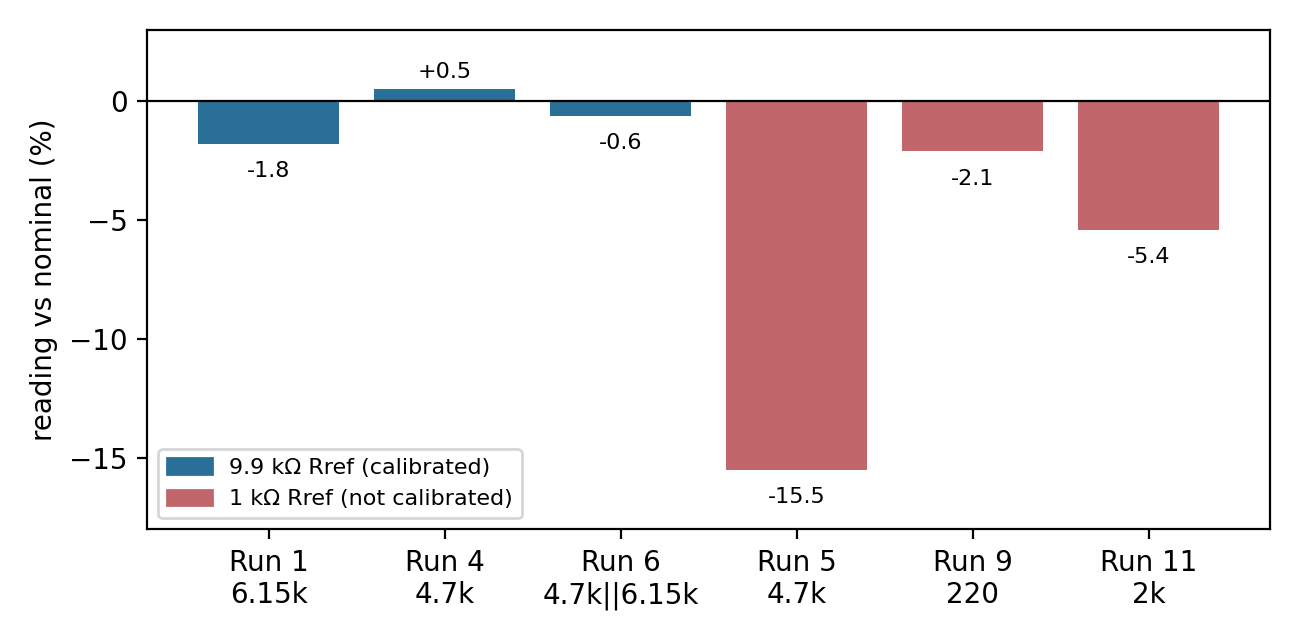
\includegraphics[width=0.75\textwidth]{fig/resistor_errors.png}
  \caption{Resistor-only runs: reading against nominal.}
\end{figure}

Observations:
\begin{itemize}
  \item On the calibrated 9.9~k$\Omega$ range, resistors read within about 2~\% (runs 1, 4, 6), and the tool chose the right model for R, R$\|$C and R+C.
  \item On the uncalibrated 1~k$\Omega$ range, errors are up to 15~\% (runs 5, 9, 11), so that range is not usable yet.
  \item Run 3: if the software $\Rref$ setting does not match the resistor on the board, the result is wrong and no error is shown. Both must be changed together.
  \item Capacitors read 6 to 33~\% below the nominal 80~nF (runs 2, 7, 8, 10, 12), and a ``200~nF'' part read about 160~nF. A series resistance appears with the capacitor: 268~$\Omega$ (run 7) and 475~$\Omega$ (run 10); in run 8 the extra resistance is about 274~$\Omega$, close to run 7. Possible causes: the capacitors are really that value and lossy (ceramic or electrolytic), or the instrument has a capacitance bias. \textbf{This was not resolved}, it needs a second capacitor of known value or an LCR meter.
\end{itemize}

\subsection{Series R + C part (``1~k$\Omega$ + 200~nF''), calibrated, 9.9~k$\Omega$ range}
\begin{center}
\begin{tabular}{lrrrr}
\toprule
Frequency & 125 Hz & 250 Hz & 500 Hz & 1000 Hz \\
\midrule
$R_s$ & 1386 $\Omega$ & 1190 $\Omega$ & 1109 $\Omega$ & 1107 $\Omega$ \\
$C_s$ & 162.9 nF & 158.6 nF & 156.3 nF & 159.0 nF \\
\bottomrule
\end{tabular}
\end{center}
Best fit: R + C series, R = 1120~$\Omega$, C = 159.4~nF, fit error 2.4~\%. C is steady across frequency, which suggests the part is about 160~nF, not 200~nF. The excess resistance above the known 1.001~k$\Omega$ divided by the reactance gives a loss factor of about 0.06, which is high for a film capacitor. Not verified against a reference meter.

\subsection{Accuracy claim}
About 1 to 2~\% on resistance on the calibrated range. Limits: $\Rref$ known only to about 1~\% (multimeter), the known-resistor calibration point (1.001~k$\Omega$) is itself a multimeter reading, and the three-point calibration residual is about 12~$\Omega$ in $Z$. A full uncertainty budget (GUM) has not been done.

\section{Simulation against hardware}
\begin{center}
\small
\begin{tabular}{p{3.6cm}p{4.6cm}p{7cm}}
\toprule
 & LTspice & Hardware \\
\midrule
Resistor / R+L accuracy & under 0.3~\% of $|\Zx|$ (ideal parts, no noise) & about 2~\% (calibrated range) \\
Offset in $\Zx$ path & none & 25 to 30~$\Omega$ before calibration \\
ADC & ideal nodes & offset 4.6~mV, noise 0.5~mV, channel gain mismatch up to 0.08~\%, sampling skew 19~$\mu$s \\
Parts & exact values & about 1~\% resistors measured by multimeter, breadboard contacts \\
\bottomrule
\end{tabular}
\end{center}

Same parts, simulation (500~Hz) against hardware:
\begin{center}
\small
\begin{tabular}{llrrlrrr}
\toprule
Part & $\Rref$ & HW run & HW reading & HW $\Delta$ & Sim case & Sim reading & Sim $\Delta$ \\
\midrule
6.15~k$\Omega$ & 9.9~k$\Omega$ & 1 & 6039.55 & $-1.8$~\% & 2 & 6149.90 & $-0.0016$~\% \\
4.7~k$\Omega$ & 9.9~k$\Omega$ & 4 & 4723.35 & +0.5~\% & 3 & 4699.93 & $-0.0015$~\% \\
2.664~k$\Omega$ & 9.9~k$\Omega$ & 6 & 2648.34 & $-0.6$~\% & 4 & 2663.97 & $-0.0012$~\% \\
220~$\Omega$ & 1~k$\Omega$ & 9 & 215.43 & $-2.1$~\% (uncal.) & 5 & 220.00 & $-0.0003$~\% \\
2~k$\Omega$ & 1~k$\Omega$ & 11 & 1891.91 & $-5.4$~\% (uncal.) & 6 & 1999.94 & $-0.0031$~\% \\
\bottomrule
\end{tabular}
\end{center}
{\small Hardware nominal values were not all measured with a multimeter (see 5.2), so part of the hardware $\Delta$ may be the part, not the instrument.}

The simulation gives the lower limit set by the circuit itself. The difference to the hardware (about 2~\%) is from component tolerance, the series offset, the AC amplitude droop at the open circuit, ADC effects and the uncertainty of the calibration standards, which are not in the LTspice model. The simulation did not predict the 25 to 30~$\Omega$ offset or the amplitude droop. The effect of capacitor losses was not simulated.

\section{Limitations}
\begin{itemize}
  \item Inductors were not tested on the hardware (none available).
  \item Source of the 25 to 30~$\Omega$ offset and the amplitude droop is not identified.
\end{itemize}

\section{Conclusion}
A divider-type impedance meter was simulated in LTspice (error under 0.3~\% with ideal parts) and built on a breadboard. After calibration it measures resistors to about 2~\% on the 9.9~k$\Omega$ range and identifies R, R$\|$C and R+C. Capacitor values and the other ranges still need verification.

\appendix
\section*{Appendix: files}
\begin{itemize}
  \item \texttt{simulation/ltspice/}: \texttt{Impedence\_Measurement.asc} (schematic), \texttt{.raw} and \texttt{.log} (results), \texttt{extract\_z.py} (reads the raw file), \texttt{results.csv} (table of $\Zx$).
  \item \texttt{hardware/}: hardware circuit drawing.
  \item \texttt{firmware/}: firmware, host tool, calibration, bring-up log (\texttt{NOTES.md}).
  \item \texttt{simulation/stage0/}, \texttt{simulation/cosim/}: Stage 0 and ngspice co-simulation.
  \item Code repository: \url{https://github.com/prabhuparth442/MEI_Impedance_Meter}
  \item \texttt{MEI\_Impedance\_Meter\_Demo.mp4} (4 min 3 s, submitted separately; captions in \texttt{video/}): side-by-side breadboard and terminal, the 12 bench runs, with captions.
\end{itemize}

\end{document}
